\section{Modeling}
\hfill \break
The data pipeline splits the feature into categorical and numerical features.

\hfill \break
We perform One hot encoding for the categorical feature and For the numerical feature We scale the data by standard scalar then do Polynomial Features (degree=6) finally We use log transformation for the data.\textbf{ As previously discussed We perform log transformation because the distance data is right skewed.}

\subsection{Results}

\begin{table}[h]
\centering
\begin{tabular}{lcc}
\toprule
\textbf{Metric} & \textbf{Train} & \textbf{Validation} \\
\midrule
RMSE & 0.4376 & 0.4427 \\
R² & 0.6968 & 0.6938 \\
\bottomrule
\end{tabular}
\caption{Performance metrics for the model}
\label{tab:performance}
\end{table}


\subsection{Lessons and future work}

\hfill \break
Having a type of version control for the data or model scores is very beneficial for error analysis and verifying assumptions. In this project, we observed the following insights:

\begin{itemize}
    \item Feature selection consistently improves model performance.
    \item Outlier removal for intra-trip duration does not improve model performance.
\end{itemize}

\hfill \break
Building a separate pipeline to estimate the speed feature and using it as an input for predicting trip duration did not significantly improve the model's performance.

\hfill \break
Linear models often exhibit high bias. Given the characteristics of this dataset, it is important to explore more complex algorithms. For heterogeneous tabular data, techniques such as XGBoost and ensemble methods can be particularly effective.


\newpage
\begin{figure}
    \centering
    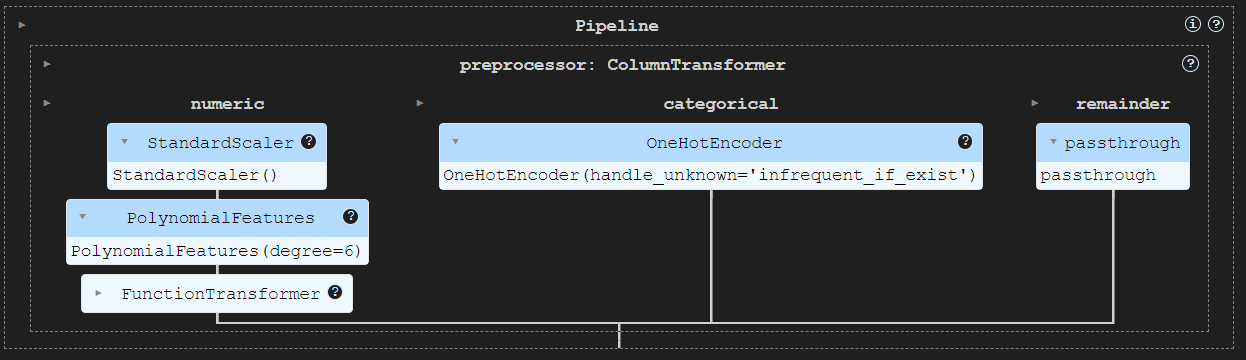
\includegraphics[width=1\linewidth]{Data Pipline.png}
    \caption{Data pipeline}
    \label{fig:Data pipeline}
\end{figure}


